\documentclass{article}
\usepackage[T1]{fontenc}
\usepackage{lmodern}
\usepackage{graphicx}
\usepackage{amsmath,amssymb}
\usepackage[a4paper,margin=2cm]{geometry}
\usepackage[absolute,overlay]{textpos}
\setlength{\TPHorizModule}{1mm}
\setlength{\TPVertModule}{1mm}
\usepackage[indonesian]{babel}
\usepackage{hyperref}
\setlength{\emergencystretch}{2em}
% unit: Halaman 9

\begin{document}

% === Halaman 9 (llm) ===

\begin{itemize}
    \item Misalnya pada kotak S pertama, masukannya:
    
    \[ 0010 \quad (\text{nilai desimal 2}) \]
    
    maka luarannya: nilai di dalam elemen ke-2:
    \[ 9 \text{ atau } 1001 \]
\end{itemize}

\vspace{5mm}

\begin{itemize}
    \item Hasil substitusi dari semua kotak S ini digabung menjadi pesan 32-bit.
\end{itemize}

% deskripsi: Tabel Kotak-S 1 yang berisi deretan angka substitusi dari indeks 0 sampai 15.
% bbox normalisasi: [0.0900, 0.5900, 0.9560, 0.6910]
\begin{textblock*}{181.86mm}(18.90mm,175.23mm)
\noindent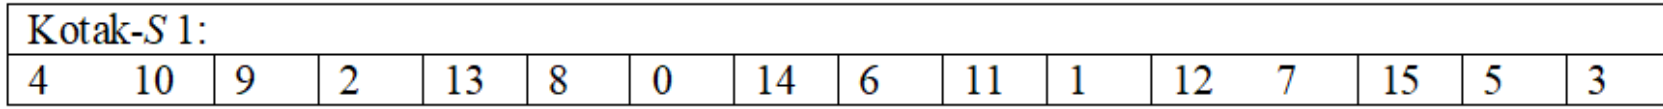
\includegraphics[width=181.86mm,height=30.00mm]{../../images/llm/page_009_img_01.png}%
\end{textblock*}

\end{document}
